% =====================================================================
%  Database and backend architecture — the typeset version of
%  HowToSetupTerminalLocally/ARCHITECTURE.md
%
%  Build:  python -m scripts.build_architecture
%  (the schema inventory is dumped from the live database first)
% =====================================================================
\documentclass[11pt,a4paper]{article}

\usepackage[T1]{fontenc}
\usepackage[utf8]{inputenc}
\usepackage[english]{babel}
\usepackage{mathpazo}
\usepackage[scaled=0.90]{helvet}
\usepackage{microtype}

\usepackage[a4paper,top=26mm,bottom=24mm,left=25mm,right=25mm]{geometry}
\usepackage{amsmath,amssymb}
\usepackage{booktabs,array,longtable,tabularx}
\usepackage{xcolor}
\usepackage{titlesec}
\usepackage{fancyhdr}
\usepackage[font=small,labelfont=bf,labelsep=period]{caption}
\usepackage{enumitem}
\usepackage{listings}
\usepackage{tikz}
\usetikzlibrary{positioning,shapes.geometric,arrows,fit,backgrounds,calc}
\usepackage[hidelinks]{hyperref}

\definecolor{navy}{HTML}{23456B}
\definecolor{ink}{HTML}{1A1A1A}
\definecolor{rule}{HTML}{C9C4BA}
\definecolor{paper}{HTML}{F7F5F0}
\definecolor{brick}{HTML}{8C3A2E}
\definecolor{moss}{HTML}{4A6B4A}

\hypersetup{
  colorlinks=true, linkcolor=navy, urlcolor=navy,
  pdftitle={Factor Terminal — database and backend architecture},
  pdfauthor={Bastian Offermann},
}

\titleformat{\section}
  {\normalfont\sffamily\large\bfseries\color{navy}}{\thesection}{0.8em}{}
\titleformat{\subsection}
  {\normalfont\sffamily\normalsize\bfseries\color{ink}}{\thesubsection}{0.7em}{}
\titlespacing*{\section}{0pt}{2.4ex plus 1ex minus .2ex}{1.1ex plus .2ex}

\pagestyle{fancy}
\fancyhf{}
\renewcommand{\headrulewidth}{0.3pt}
\renewcommand{\headrule}{\hbox to\headwidth{\color{rule}%
  \leaders\hrule height \headrulewidth\hfill}}
\fancyhead[L]{\footnotesize\sffamily\color{navy}Factor Terminal · database and backend architecture}
\fancyhead[R]{\footnotesize\sffamily\color{navy}\thepage}

\setlength{\parskip}{0.6ex}
\setlength{\parindent}{0pt}
\renewcommand{\arraystretch}{1.18}

\newcommand{\code}[1]{\texttt{\small #1}}

% A rule-bounded note for the decisions that would otherwise be lost.
\newsavebox{\notebox}
\newenvironment{designnote}[1]
  {\par\vspace{1.6ex}%
   \begin{lrbox}{\notebox}\begin{minipage}{\textwidth}%
   {\color{rule}\rule{\textwidth}{0.4pt}}\par\vspace{0.7ex}
   {\small\sffamily\bfseries\color{navy}#1}\par\vspace{0.35ex}
   \small\itshape}
  {\par\vspace{0.7ex}\noindent{\color{rule}\rule{\textwidth}{0.4pt}}%
   \end{minipage}\end{lrbox}%
   \noindent\usebox{\notebox}\par\vspace{1.6ex}}

\lstset{
  basicstyle=\ttfamily\footnotesize,
  keywordstyle=\color{navy}\bfseries,
  commentstyle=\color{moss}\itshape,
  stringstyle=\color{brick},
  backgroundcolor=\color{paper},
  frame=single, rulecolor=\color{rule}, framesep=6pt,
  xleftmargin=2pt, xrightmargin=2pt,
  breaklines=true, showstringspaces=false,
  columns=fullflexible, aboveskip=1.4ex, belowskip=1.4ex,
}

% ---------------------------------------------------------------------
%  Shared TikZ vocabulary for both workflow figures.
% ---------------------------------------------------------------------
\tikzset{
  font=\sffamily\scriptsize,
  >=stealth,
  src/.style   = {draw=rule, fill=white, rounded corners=1pt, align=center,
                  minimum height=8mm, inner xsep=5pt, text=ink},
  job/.style   = {draw=navy!55, fill=navy!7, rounded corners=1pt, align=center,
                  minimum height=9mm, inner xsep=5pt, text=ink},
  store/.style = {cylinder, shape border rotate=90, aspect=0.10,
                  draw=moss!70, fill=moss!8, align=center, text=ink,
                  inner xsep=5pt, inner ysep=3pt},
  ui/.style    = {draw=brick!55, fill=brick!7, rounded corners=1pt, align=center,
                  minimum height=8mm, inner xsep=5pt, text=ink},
  pure/.style  = {draw=navy, dashed, fill=white, rounded corners=1pt,
                  align=center, minimum height=9mm, inner xsep=5pt, text=ink},
  flow/.style  = {->, draw=navy!65, line width=0.55pt},
  back/.style  = {->, draw=brick!70, line width=0.55pt, dashed},
  imp/.style   = {->, draw=navy!45, line width=0.5pt, dotted},
  tag/.style   = {font=\sffamily\scriptsize, text=ink, fill=white,
                  inner xsep=2pt, inner ysep=1pt},
}

% Generated by scripts/build_architecture.py -- do not edit by hand.
\newcommand{\schemaTables}{29}
\newcommand{\schemaViews}{3}
\newcommand{\schemaIndexes}{55}
\newcommand{\schemaIndexCount}{55}
\newcommand{\schemaSize}{687 MB}
\newcommand{\apiRouters}{8}
\newcommand{\apiEndpoints}{39}

\newcommand{\schemaInventory}{%
\begin{center}\small
\begin{longtable}{@{}lp{0.40\textwidth}rr@{}}
\toprule
\textbf{Table} & \textbf{Primary key} & \textbf{Rows} & \textbf{Size} \\
\midrule \endfirsthead
\toprule
\textbf{Table} & \textbf{Primary key} & \textbf{Rows} & \textbf{Size} \\
\midrule \endhead
\bottomrule \endfoot
\multicolumn{4}{@{}l}{\textbf{\color{navy}Reference}} \\
\quad \code{ref\_factor\_block} & {\footnotesize \code{block\_id}} & 9 & 64 kB \\
\quad \code{ref\_factor} & {\footnotesize \code{factor\_id}} & 40 & 112 kB \\
\quad \code{ref\_instrument} & {\footnotesize \code{instrument\_id}} & 204 & 224 kB \\
\quad \code{ref\_level\_series} & {\footnotesize \code{series\_id}} & 53 & 88 kB \\
\quad \code{ref\_calendar} & {\footnotesize \code{date}} & 8,198 & 1984 kB \\
\quad \code{ref\_security} & {\footnotesize \code{instrument\_id}} & 9,434 & 2728 kB \\
\addlinespace
\multicolumn{4}{@{}l}{\textbf{\color{navy}Inputs}} \\
\quad \code{fact\_input\_return} & {\footnotesize \code{instrument\_id, date}} & 1,016,170 & 241 MB \\
\quad \code{fact\_input\_level} & {\footnotesize \code{series\_id, date}} & 253,513 & 53 MB \\
\quad \code{fact\_input\_fx} & {\footnotesize \code{ccy, date}} & 274,485 & 39 MB \\
\quad \code{fact\_reference\_factor} & {\footnotesize \code{dataset, factor, date}} & 452,553 & 129 MB \\
\addlinespace
\multicolumn{4}{@{}l}{\textbf{\color{navy}Factors}} \\
\quad \code{fact\_factor\_return} & {\footnotesize \code{factor\_id, date}} & 200,147 & 48 MB \\
\quad \code{fact\_factor\_build} & {\footnotesize \code{factor\_id, built\_at}} & 0 & 16 kB \\
\quad \code{fact\_series\_diagnostics} & {\footnotesize \code{series\_key, series\_type, as\_of\_date, window\_days}} & 893 & 552 kB \\
\addlinespace
\multicolumn{4}{@{}l}{\textbf{\color{navy}Estimation}} \\
\quad \code{dim\_model\_spec} & {\footnotesize \code{spec\_id}} & 13 & 64 kB \\
\quad \code{fact\_loading} & {\footnotesize \code{spec\_id, instrument\_id, window\_end, factor\_id}} & 390,184 & 150 MB \\
\quad \code{fact\_regression\_meta} & {\footnotesize \code{spec\_id, instrument\_id, window\_end}} & 11,599 & 6160 kB \\
\addlinespace
\multicolumn{4}{@{}l}{\textbf{\color{navy}Covariance}} \\
\quad \code{fact\_factor\_cov} & {\footnotesize \code{spec\_id, as\_of\_date, method, factor\_i, factor\_j}} & 0 & 24 kB \\
\quad \code{fact\_factor\_cov\_meta} & {\footnotesize \code{spec\_id, as\_of\_date, method}} & 0 & 16 kB \\
\quad \code{fact\_specific\_risk} & {\footnotesize \code{spec\_id, instrument\_id, as\_of\_date}} & 0 & 24 kB \\
\quad \code{fact\_residual\_pca} & {\footnotesize \code{spec\_id, as\_of\_date, component}} & 0 & 16 kB \\
\addlinespace
\multicolumn{4}{@{}l}{\textbf{\color{navy}Risk}} \\
\quad \code{fact\_risk\_forecast} & {\footnotesize \code{spec\_id, instrument\_id, as\_of\_date, horizon\_days, cov\_method}} & 8,322 & 4928 kB \\
\quad \code{fact\_risk\_contribution} & {\footnotesize \code{spec\_id, instrument\_id, as\_of\_date, block\_id}} & 0 & 16 kB \\
\quad \code{fact\_risk\_backtest} & {\footnotesize \code{spec\_id, instrument\_id, sample\_start, sample\_end, horizon\_days, cov\_method}} & 18 & 32 kB \\
\addlinespace
\multicolumn{4}{@{}l}{\textbf{\color{navy}Operations}} \\
\quad \code{etl\_run} & {\footnotesize \code{run\_id}} & 92 & 88 kB \\
\quad \code{etl\_item\_state} & {\footnotesize \code{job, item\_key}} & 502 & 336 kB \\
\quad \code{stage\_return} & {\footnotesize \code{run\_id, instrument\_id, date}} & 0 & 16 kB \\
\quad \code{stage\_level} & {\footnotesize \code{run\_id, series\_id, date}} & 0 & 16 kB \\
\addlinespace
\multicolumn{4}{@{}l}{\textbf{\color{navy}Assistant}} \\
\quad \code{chat\_thread} & {\footnotesize \code{thread\_id}} & 7 & 48 kB \\
\quad \code{chat\_message} & {\footnotesize \code{thread\_id, seq}} & 18 & 128 kB \\
\end{longtable}
\emph{29 tables, 3 views, 55 indexes, 687 MB in total on a fully loaded install.}
\end{center}}

\newcommand{\schemaLayers}{%
\begin{center}\small
\begin{tabular}{@{}lrrl@{}}
\toprule
\textbf{Layer} & \textbf{Rows} & \textbf{Size} & \textbf{Refreshed} \\
\midrule
Instrument returns & 1,016,170 & 241 MB & nightly, incremental \\
Reference factors & 452,553 & 129 MB & nightly \\
FX & 274,485 & 39 MB & nightly \\
Level series & 253,513 & 53 MB & nightly \\
Factor returns & 200,147 & 48 MB & nightly, rebuilt \\
Loadings & 390,184 & 150 MB & on demand, per spec\_id \\
Regression diagnostics & 11,599 & 6160 kB & on demand, per spec\_id \\
Risk forecasts & 8,322 & 4928 kB & on demand, per spec\_id \\
Security catalogue & 9,434 & 2728 kB & nightly \\
\midrule
\textbf{Total} & & \textbf{687 MB} & $\approx$\,2 minutes nightly \\
\bottomrule
\end{tabular}
\end{center}}


% =====================================================================
\begin{document}

% ---------------------------------------------------------------- title
\thispagestyle{empty}
\vspace*{0.4cm}
{\raggedright
{\color{rule}\rule{\textwidth}{0.8pt}}\\[1.8ex]
{\sffamily\footnotesize\color{brick}\MakeUppercase{Reference}\par}
\vspace{0.8ex}
{\sffamily\LARGE\bfseries\color{navy} Database and backend architecture\par}
\vspace{1.0ex}
{\sffamily\large\color{ink} What the setup creates, and how the backend uses it\par}
\vspace{1.6ex}
{\color{rule}\rule{\textwidth}{0.8pt}}\\[1.8ex]
{\small Bastian Offermann \quad·\quad September 2026 \quad·\quad
 \code{bastofferm/factor-terminal}\par}
}

\vspace{2.0ex}

\begin{designnote}{What this document is}
The install manual is \code{HowToSetupTerminalLocally/README.md}; this is the
reference behind it --- the schema table by table, the layering of the backend,
and the contract the warehouse has to satisfy. For the statistics rather than the
plumbing, see \emph{factor-model-paper.pdf}: §7 is the operating workflow, §8 the
architecture at a higher level, and Appendix A every statistical procedure in the
form it is implemented.
\end{designnote}

\vspace{0.6ex}
{\hypersetup{linkcolor=ink}\small\tableofcontents}

\newpage

% =====================================================================
\section{The shape of the system}
\label{sec:shape}

\begin{figure}[htbp]
\centering
\resizebox{\textwidth}{!}{%
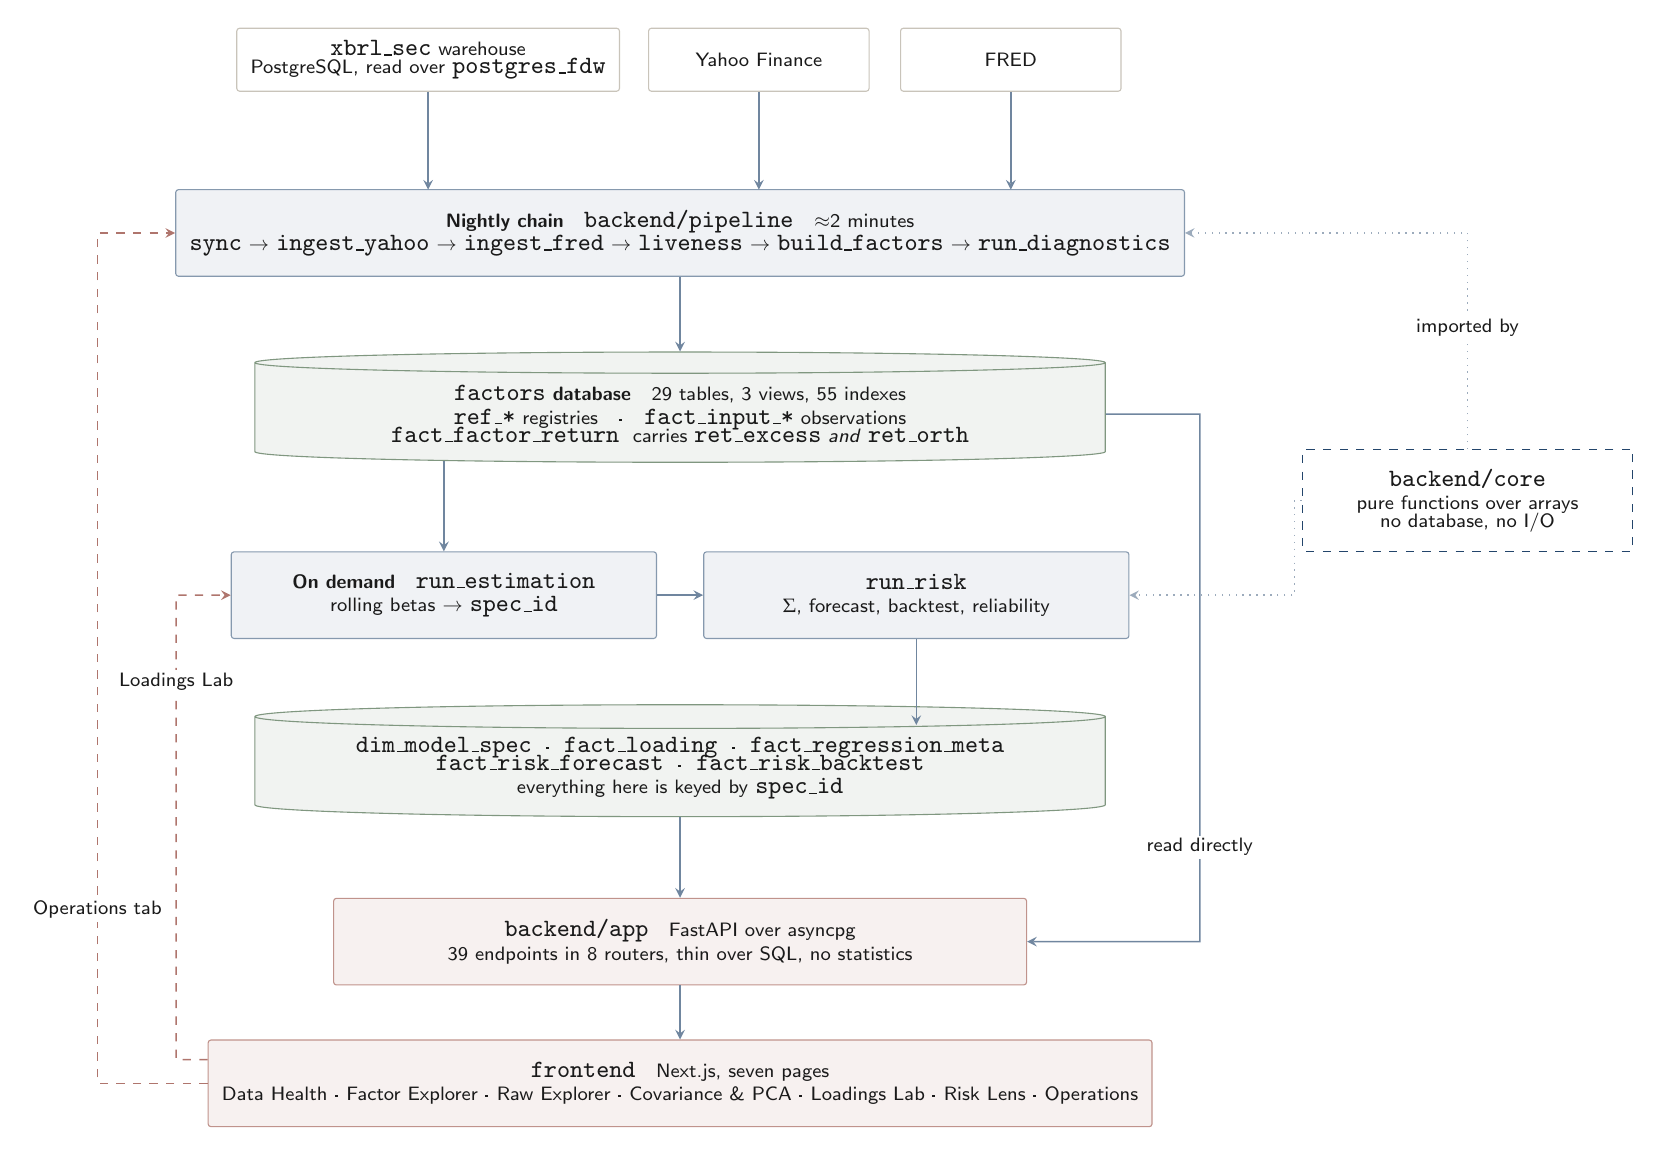
\begin{tikzpicture}[store/.append style={aspect=0.035}]

% ---- sources (y = 0) --------------------------------------------------
\node[src, minimum width=48mm] at (-32mm, 0)
  (wh) {\code{xbrl\_sec} warehouse\\[-1.5pt]\scriptsize PostgreSQL, read over \code{postgres\_fdw}};
\node[src, minimum width=28mm] at ( 10mm, 0) (yh) {Yahoo Finance};
\node[src, minimum width=28mm] at ( 42mm, 0) (fr) {FRED};

% ---- nightly chain (y = -22) ------------------------------------------
\node[job, minimum width=114mm, minimum height=11mm] at (0mm, -22mm) (night)
  {\textbf{Nightly chain} \ \ \code{backend/pipeline} \ \ \scriptsize$\approx$2 minutes\\[0.5pt]\scriptsize
   \code{sync} $\rightarrow$ \code{ingest\_yahoo} $\rightarrow$
   \code{ingest\_fred} $\rightarrow$ \code{liveness} $\rightarrow$
   \code{build\_factors} $\rightarrow$ \code{run\_diagnostics}};

% ---- the store (y = -45) ----------------------------------------------
\node[store, minimum width=108mm, minimum height=14mm] at (0mm, -45mm) (db)
  {\textbf{\code{factors} database} \ \ \scriptsize\schemaTables{} tables, \schemaViews{} views, \schemaIndexes{} indexes\\[0.5pt]\scriptsize
   \code{ref\_*} registries \ \ · \ \ \code{fact\_input\_*} observations\\[-1.5pt]\scriptsize
   \code{fact\_factor\_return} \ carries \code{ret\_excess} \emph{and} \code{ret\_orth}};

% ---- on demand (y = -68) ----------------------------------------------
\node[job, minimum width=54mm, minimum height=11mm] at (-30mm, -68mm) (est)
  {\textbf{On demand} \ \ \code{run\_estimation}\\[0.5pt]\scriptsize
   rolling betas $\rightarrow$ \code{spec\_id}};
\node[job, minimum width=54mm, minimum height=11mm] at ( 30mm, -68mm) (risk)
  {\code{run\_risk}\\[0.5pt]\scriptsize $\Sigma$, forecast, backtest, reliability};

\node[store, minimum width=108mm, minimum height=13mm] at (0mm, -90mm) (cache)
  {\code{dim\_model\_spec} \ · \ \code{fact\_loading} \ · \ \code{fact\_regression\_meta}\\[-1.5pt]
   \code{fact\_risk\_forecast} \ · \ \code{fact\_risk\_backtest}\\[0.5pt]\scriptsize
   everything here is keyed by \code{spec\_id}};

% ---- pure core, off to the right --------------------------------------
\node[pure, minimum width=42mm, minimum height=13mm] at (100mm, -56mm) (core)
  {\textbf{\code{backend/core}}\\[0.5pt]\scriptsize
   pure functions over arrays\\[-1.5pt]\scriptsize no database, no I/O};

% ---- serve ------------------------------------------------------------
\node[ui, minimum width=88mm, minimum height=11mm] at (0mm, -112mm) (api)
  {\textbf{\code{backend/app}} \ \ FastAPI over asyncpg\\[0.5pt]\scriptsize
   \apiEndpoints{} endpoints in \apiRouters{} routers, thin over SQL, no statistics};
\node[ui, minimum width=114mm, minimum height=11mm] at (0mm, -130mm) (fe)
  {\textbf{\code{frontend}} \ \ Next.js, seven pages\\[0.5pt]\scriptsize
   Data Health · Factor Explorer · Raw Explorer · Covariance \& PCA ·
   Loadings Lab · Risk Lens · Operations};

% ---- forward edges ----------------------------------------------------
\draw[flow] (wh.south) -- ++(0,-5mm) -| (-32mm,-16.5mm);
\draw[flow] (yh.south) -- ++(0,-5mm) -| ( 10mm,-16.5mm);
\draw[flow] (fr.south) -- ++(0,-5mm) -| ( 42mm,-16.5mm);
\draw[flow] (night) -- (db);
\draw[flow] (-30mm,-51mm) -- (est.north);
\draw[flow] (est) -- (risk);
\draw[flow] (risk.south) -- ++(0,-8mm) -| (30mm,-84.5mm);
\draw[flow] (cache) -- (api);
\draw[flow] (api) -- (fe);

% the store is read by the API directly as well as through the cache
\draw[flow] (db.east) -- (66mm,-45mm) -- (66mm,-112mm) -- (api.east);
\node[tag] at (66mm,-100mm) {read directly};

% ---- imports ----------------------------------------------------------
\draw[imp] (core.west) -- (78mm,-56mm) -- (78mm,-68mm) -- (risk.east);
\draw[imp] (core.north) -- (100mm,-22mm) -- (night.east);
\node[tag] at (100mm,-34mm) {imported by};

% ---- the interface reaching back --------------------------------------
\draw[back] (fe.west) -- (-74mm,-130mm) -- (-74mm,-22mm) -- (night.west);
\node[tag] at (-74mm,-108mm) {Operations tab};
\draw[back] ($(fe.west)+(0,3mm)$) -- (-64mm,-127mm) -- (-64mm,-68mm) -- (est.west);
\node[tag] at (-64mm,-79mm) {Loadings Lab};

\end{tikzpicture}}
\caption{The system end to end. Solid arrows are data moving forward, dotted
arrows are imports, dashed arrows are the interface reaching back into the
pipeline. Drums are storage. Two properties are load-bearing and are drawn rather
than described: \code{backend/core} has no edge into the database, and the store in
the middle is the only state the two computation paths share.}
\label{fig:shape}
\end{figure}

Two rules hold the design together.

\textbf{\code{backend/core} touches nothing.} Every statistical routine is a pure
function over NumPy arrays: no database handle, no configuration lookup, no logging
side effect. That is what makes the accuracy claims testable --- a test feeds each
routine a process whose answer is known analytically and asserts it gets there,
with no fixture and no database. The alternative, statistics computed inside the
query that fetches the data, would make every claim checkable only by reading it.

\textbf{The database is the only shared state.} \code{backend/pipeline} writes it,
\code{backend/app} reads it, and neither calls the other. A refresh that fails
leaves yesterday's panel intact and every cached specification still readable.

% =====================================================================
\section{Naming convention}

The prefix says what a table is for, and therefore who is allowed to write it.

\begin{table}[htbp]
\centering\small
\begin{tabularx}{\textwidth}{@{}lXll@{}}
\toprule
\textbf{Prefix} & \textbf{Meaning} & \textbf{Written by} & \textbf{Example} \\
\midrule
\code{ref\_} & Reference data: what exists, and how to treat it & \code{sync}, \code{seed} & \code{ref\_factor} \\
\code{fact\_} & Observations and results, on a natural key & pipeline jobs & \code{fact\_factor\_return} \\
\code{dim\_} & A dimension other tables key into & \code{run\_estimation} & \code{dim\_model\_spec} \\
\code{stage\_} & Scratch space inside one job's transaction & ingest jobs & \code{stage\_return} \\
\code{etl\_} & Operational state: what ran, when, how it went & every job & \code{etl\_run} \\
\code{v\_} & Views. No storage; read by the API & --- & \code{v\_data\_health} \\
\code{warehouse\_sec.} & Foreign tables. \textbf{Read-only, never written} & --- & \code{warehouse\_sec.fact\_macro} \\
\bottomrule
\end{tabularx}
\end{table}

% =====================================================================
\section{Migrations}

Fifteen files in \code{sql/}, applied in order by a runner that fails fast: a
migration error aborts with a non-zero exit code rather than logging and
continuing, so a partially applied schema can never be mistaken for a good one.
Every file is idempotent --- \code{CREATE TABLE IF NOT EXISTS},
\code{CREATE OR REPLACE VIEW} --- so re-running is safe, and
\code{create\_tables.py} re-running on a complete database reports
\emph{no new objects} for all fifteen.

\begin{table}[htbp]
\centering\small
\begin{tabularx}{\textwidth}{@{}lX@{}}
\toprule
\textbf{Migration} & \textbf{Creates} \\
\midrule
\code{001\_reference.sql} & \code{ref\_factor\_block}, \code{ref\_instrument}, \code{ref\_factor}, \code{ref\_calendar} \\
\code{002\_inputs.sql} & \code{fact\_input\_return}, \code{fact\_input\_level}, \code{ref\_level\_series}, \code{fact\_input\_fx}, \code{fact\_reference\_factor} \\
\code{003\_factors.sql} & \code{fact\_factor\_return}, \code{fact\_factor\_build} \\
\code{004\_diagnostics.sql} & \code{fact\_series\_diagnostics}, view \code{v\_series\_diagnostics\_latest} \\
\code{005\_estimation.sql} & \code{dim\_model\_spec}, \code{fact\_loading}, \code{fact\_regression\_meta}, view \code{v\_regression\_quality} \\
\code{006\_covariance.sql} & \code{fact\_factor\_cov}, \code{fact\_factor\_cov\_meta}, \code{fact\_specific\_risk}, \code{fact\_residual\_pca} \\
\code{007\_risk.sql} & \code{fact\_risk\_forecast}, \code{fact\_risk\_contribution}, \code{fact\_risk\_backtest} \\
\code{008\_ops.sql} & \code{etl\_run}, \code{etl\_item\_state}, \code{stage\_return}, \code{stage\_level}, view \code{v\_data\_health} \\
\code{009\_fdw.sql} & extension \code{postgres\_fdw}, server \code{warehouse} \\
\code{010\_fdw\_import.sql} & schema \code{warehouse\_sec} with 11 foreign tables \\
\code{011\_risk\_reliability.sql} & partial index over reliable forecasts \\
\code{012\_chat.sql} & \code{chat\_thread}, \code{chat\_message} \\
\code{013\_beta\_overlap.sql} & \code{fact\_regression\_meta.beta\_overlap} \\
\code{014\_block\_names\_en.sql} & block name corrections \\
\code{015\_security\_catalogue.sql} & \code{ref\_security} \\
\bottomrule
\end{tabularx}
\end{table}

\begin{designnote}{Why 009 and 010 are two files}
\code{IMPORT FOREIGN SCHEMA} is not idempotent --- dropping and re-importing is how
a schema change on the warehouse side gets picked up --- and the \code{USER MAPPING}
that has to exist between them carries a password. A migration with a credential in
it is not a thing to commit, so the mapping is created by \code{apply\_schema.py}
from \code{PGPASSWORD} at apply time.
\end{designnote}

% =====================================================================
\section{The tables}

\schemaInventory{}

\subsection{Reference: what exists}

\code{ref\_factor.orthogonalize\_against} is a PostgreSQL \code{text} array of
factor ids. It
encodes the block hierarchy, and because every target sits at a lower level the
graph is acyclic by construction and the panel builds in one pass.

\code{ref\_calendar} is the trading calendar, and \textbf{crypto is excluded from
it}. Crypto prices seven days a week; included, it added 1{,}229 weekend rows on
which every other factor is missing, which made 252-row estimation windows span
fewer than 252 trading days and pushed equity factors below the coverage threshold
in the covariance matrix. The defect surfaced only because the matrix endpoint
began returning 8 factors where 39 were expected.

\code{ref\_security} is materialised nightly rather than derived on read: computing
it means aggregating two price tables of fifteen million rows apiece, about eight
seconds per keystroke in a search box.

\subsection{Inputs: raw observations}

\code{fact\_input\_return} carries \code{source} (\code{warehouse} or
\code{yahoo}) and \code{currency}, so a row's provenance is a column rather than an
inference. Securities pulled on demand are converted to the base currency at
ingestion --- $r^{\mathrm{USD}} = r^{\mathrm{local}} + r^{\mathrm{fx}}$ in logs ---
because storing a local-currency return and regressing it on dollar-denominated
factors makes the currency appear as a spurious exposure.

\code{fact\_reference\_factor} holds Fama-French and AQR series. They lag by one to
two months and can never drive a daily model; they exist to confirm that a
construction measures what its name claims.

\subsection{Factors: one table, two panels}

\begin{lstlisting}[language=SQL]
fact_factor_return(factor_id, date, ret_excess, ret_orth, ...)
\end{lstlisting}

\code{ret\_excess} is the raw excess return; \code{ret\_orth} is the
block-hierarchy residual, fitted causally on a trailing 504-day window refitted
every 21 days. Storing both rather than deriving one on read is what lets a
specification declare which panel it was estimated on and be scored against the
matching covariance.

\begin{designnote}{The constraint behind the second column}
Portfolio risk is $\beta'\Sigma\beta$, so $\Sigma$ must be the covariance of
exactly the series the $\beta$s refer to. Pairing one panel's betas with the
other's covariance produces a wrong number with no error raised and nothing
implausible to give it away. \code{run\_risk} reads the specification's own panel
flag for that reason. It did not always, and every predicted volatility a
raw-panel specification produced was silently wrong until it did.
\end{designnote}

\code{fact\_series\_diagnostics} has 42 columns --- every statistic the stationarity
battery produces, mapping one-to-one onto the \code{Diagnostics} dataclass in
\code{backend/core/stationarity.py}. The view
\code{v\_series\_diagnostics\_latest} picks the newest row per series and window.

\subsection{Estimation: keyed by \code{spec\_id}}

\code{spec\_id} is the first 32 hex characters of a SHA-256 over the canonical JSON
of every parameter that changes the answer: window, step, estimator, weighting,
half-life, ridge $\lambda$, Dimson lags, winsorisation, HAC lags, minimum
observations, the sorted factor set, and the factor panel.

Two things follow. Re-requesting a view an analyst has already seen is a table read
rather than several hundred regressions. And any stored number is reproducible: the
specification behind it can be recovered from its identifier and re-run --- which
is what the Loadings Lab's run inspector does, unpacking a \code{spec\_id} back
into the parameters that produced it.

\code{fact\_regression\_meta} carries 23 columns of per-window diagnostics: $R^2$,
adjusted $R^2$, $F$ and its $p$-value, RMSE, residual volatility, Durbin-Watson,
condition number, maximum VIF, Ljung-Box and ARCH-LM on the residuals, the $L_1$
beta shift, the correlation with the previous window, and the size of the
overlapping factor set. The last three are the drift alert; the condition number
and the maximum VIF are what the reliability gate reads.

\subsection{Covariance and risk}

Forecasts built on ill-conditioned windows are \textbf{stored, flagged and excluded
from scoring} --- not silently dropped, and not silently used.
\code{is\_reliable} and \code{unreliable\_reason} are columns for that reason, and
\code{011\_risk\_reliability.sql} adds a partial index so the scored subset is cheap
to select.

\code{fact\_risk\_backtest} has 31 columns: bias ratio and bias statistic,
Mincer-Zarnowitz $\alpha$, $\beta$, their $p$-values, the joint $p$ and $R^2$, and
Kupiec and Christoffersen at both the 95\% and 99\% levels.

\subsection{Operations and the assistant}

\code{etl\_run} holds one row per job invocation --- mode, scope, status, rows in
and out, failure count, error --- and \code{etl\_item\_state} the per-item state, so
a partial failure is resumable rather than a restart. \code{v\_data\_health} joins
these into what the Data Health page and the Operations tab read.

\code{chat\_thread} and \code{chat\_message} store every exchange \emph{together
with the page snapshot the answer was grounded in}, which is what lets a statement
be checked later against the numbers that were on screen when it was made.

% =====================================================================
\section{Indexes}

\schemaIndexCount{} indexes. Beyond the primary keys, three patterns.

\textbf{Date lookups.} Every \code{fact\_*} time series has an index on
\code{date} alone, for ``everything as of this day'' queries --- the covariance
matrix and the data-health banner both need them.

\textbf{Composite lookup keys.} \code{idx\_loading\_lookup} and
\code{idx\_reg\_meta\_lookup} cover \code{(spec\_id, instrument\_id, window\_end)},
which is the access path for every Loadings Lab request.
\code{idx\_loading\_factor} covers the transpose --- one factor across every window
--- for the beta-path charts.

\textbf{Partial indexes.} \code{idx\_risk\_forecast\_reliable} covers only the rows
where \code{is\_reliable}, because scoring reads exactly that subset and it is the
majority of risk queries.

\code{ref\_security} carries four, including
\code{lower(name) text\_pattern\_ops} for the search box ---
\code{text\_pattern\_ops} so a prefix \code{LIKE} can use the index under any
collation. Scanning 9{,}434 rows per keystroke would be visible latency.

% =====================================================================
\section{The warehouse contract}
\label{sec:contract}

Eleven foreign tables are imported into \code{warehouse\_sec}. If you are pointing
the model at your own database, this is what it has to provide in a schema called
\code{sec}.

\begin{table}[htbp]
\centering\small
\begin{tabularx}{\textwidth}{@{}lXl@{}}
\toprule
\textbf{Foreign table} & \textbf{Columns read} & \textbf{Used for} \\
\midrule
\code{dim\_cross\_asset} & \code{ticker, name, asset\_class} & seeds \code{ref\_instrument} \\
\code{fact\_cross\_asset} & \code{ticker, date, close, adj\_close, return, log\_return, volume, currency} & fund, index, futures, FX and crypto prices \\
\code{ref\_macro\_series} & \code{series\_id, name} & names for \code{ref\_level\_series} \\
\code{fact\_macro} & \code{series\_id, date, value} & yields, spreads, policy rates \\
\code{fact\_fx} & \code{ccy, fx\_date, usd\_per\_unit} & base-currency conversion \\
\code{fact\_fama\_french} & \code{dataset, factor, date, return\_pct, value, return\_log} & reference factors \\
\code{dim\_ff\_dataset} & --- & dataset registry \\
\code{fact\_prices\_us} & \code{ticker, date, close, adj\_close, return, log\_return, volume} & US equities, on demand \\
\code{fact\_prices\_jp} & as above & Japanese equities, on demand \\
\code{dim\_company\_us} & \code{primary\_ticker, name, exchange, gics\_sector\_name} & catalogue names \\
\code{dim\_company\_jp} & \code{primary\_ticker, name, gics\_sector\_name} & catalogue names \\
\bottomrule
\end{tabularx}
\end{table}

Two quirks the sync code handles, worth knowing if you are building a substitute.

\textbf{\code{fact\_fama\_french} carries two conventions in one table.} The Ken
French loader fills \code{return\_pct} in percent ($0.5 = +0.5\%$); the AQR loader
fills only \code{value}, as a decimal ($0.005 = +0.5\%$). Both are normalised to
percent on the way in. Reading only \code{return\_pct} makes every AQR series
arrive NULL and drop silently out of the validation.

\textbf{\code{dim\_company\_jp.primary\_ticker} carries the Tokyo suffix}
(\code{7203.T}) while \code{fact\_prices\_jp.ticker} does not (\code{7203}).
Joining them directly matched 17 names out of 3{,}878; the catalogue query joins on
\code{d.primary\_ticker IN (c.ticker, c.ticker || '.T')}.

The wrapper is configured with \code{fetch\_size '50000'} and
\code{use\_remote\_estimate 'true'}: large batches because the transfers are bulk,
and remote estimates because without them the planner assumes default selectivity
for foreign tables and chooses a nested loop over a million rows.

% =====================================================================
\section{The backend}

\begin{lstlisting}
backend/
  core/         2,309 lines. Pure functions over arrays. No I/O.
                stationarity - transforms - orthogonalize - regression
                covariance - risk - distribution - summary
  pipeline/     4,498 lines. Jobs. May touch the database (psycopg2).
                sync - ingest_yahoo - ingest_fred - build_factors
                run_diagnostics - run_estimation - run_risk - scheduler
                formula - factor_defs - seed - dbsync - apply_schema
  app/          3,726 lines. FastAPI over asyncpg. No statistics.
                main - db - settings - runs - provenance
                routers/{meta,factors,raw,matrix,loadings,risk,ops,chat}
                ai/{providers,corpus,context,prompts}
  tests/        4,252 lines, 352 tests
\end{lstlisting}

\subsection{Two drivers, deliberately}

\textbf{asyncpg} in the API: a connection pool sized by \code{POOL\_MIN} and
\code{POOL\_MAX}, a \code{statement\_timeout} applied per session through
\code{server\_settings}, and async all the way down so one slow query does not
block the event loop.

\textbf{psycopg2} in the pipeline: the jobs are synchronous, long-running and
transactional, and \code{execute\_values} for bulk insert is what makes a
million-row sync finish in seconds. Async would buy nothing in a batch job and
would complicate the transaction boundaries that make a partial failure resumable.

\begin{designnote}{A numeric that arrives as a string}
asyncpg renders PostgreSQL \code{numeric} as a JSON string. An endpoint returning
\code{EXTRACT(EPOCH ...)} therefore handed the browser \code{"12.4"} where it
expected a number, \code{.toFixed()} threw inside render, and the whole page went
blank with no error in the network tab. Cast to \code{::double precision} in the
query.
\end{designnote}

\subsection{Request lifecycle}

\begin{figure}[htbp]
\centering
\resizebox{0.96\textwidth}{!}{%
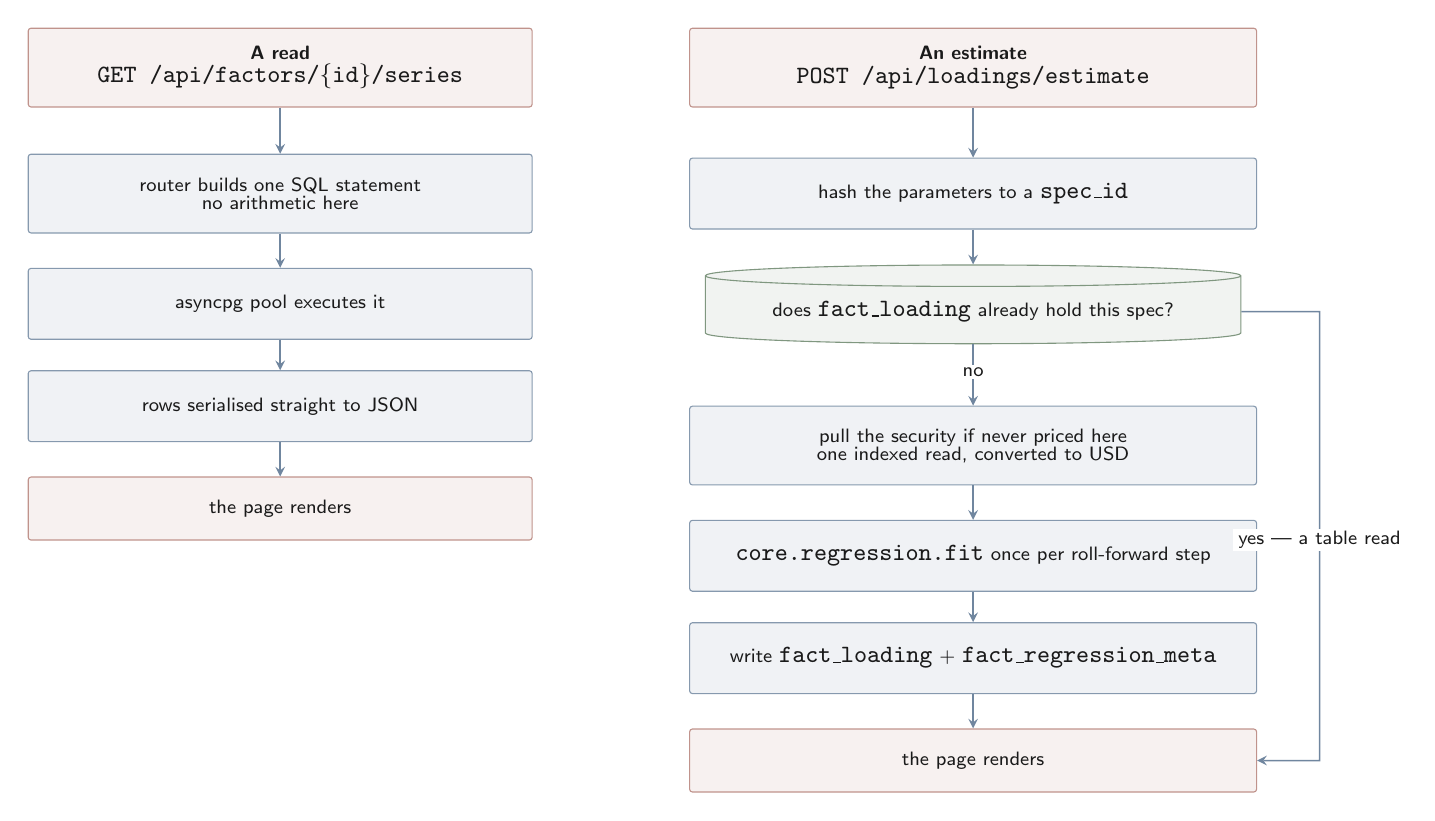
\begin{tikzpicture}[store/.append style={aspect=0.05}]

% ---------------- read path -------------------------------------------
\node[ui, minimum width=64mm, minimum height=10mm] at (-42mm, 0) (r0)
  {\textbf{A read}\\[0.5pt]\code{GET /api/factors/\{id\}/series}};
\node[job, minimum width=64mm, minimum height=10mm] at (-42mm, -16mm) (r1)
  {router builds one SQL statement\\[-1.5pt]\scriptsize no arithmetic here};
\node[job, minimum width=64mm] at (-42mm, -30mm) (r2)
  {asyncpg pool executes it};
\node[job, minimum width=64mm] at (-42mm, -43mm) (r3)
  {rows serialised straight to JSON};
\node[ui, minimum width=64mm] at (-42mm, -56mm) (r4)
  {the page renders};

\draw[flow] (r0) -- (r1);
\draw[flow] (r1) -- (r2);
\draw[flow] (r2) -- (r3);
\draw[flow] (r3) -- (r4);

% ---------------- estimate path ---------------------------------------
\node[ui, minimum width=72mm, minimum height=10mm] at (46mm, 0) (e0)
  {\textbf{An estimate}\\[0.5pt]\code{POST /api/loadings/estimate}};
\node[job, minimum width=72mm] at (46mm, -16mm) (e1)
  {hash the parameters to a \code{spec\_id}};
\node[store, minimum width=68mm, minimum height=10mm] at (46mm, -31mm) (e2)
  {does \code{fact\_loading} already hold this spec?};
\node[job, minimum width=72mm, minimum height=10mm] at (46mm, -48mm) (e3)
  {pull the security if never priced here\\[-1.5pt]\scriptsize one indexed read, converted to USD};
\node[job, minimum width=72mm] at (46mm, -62mm) (e4)
  {\code{core.regression.fit} once per roll-forward step};
\node[job, minimum width=72mm] at (46mm, -75mm) (e5)
  {write \code{fact\_loading} + \code{fact\_regression\_meta}};
\node[ui, minimum width=72mm] at (46mm, -88mm) (e6)
  {the page renders};

\draw[flow] (e0) -- (e1);
\draw[flow] (e1) -- (e2);
\draw[flow] (e2) -- node[tag, pos=0.45] {no} (e3);
\draw[flow] (e3) -- (e4);
\draw[flow] (e4) -- (e5);
\draw[flow] (e5) -- (e6);

% the cache hit short-circuits everything below it
\draw[flow] (e2.east) -- (90mm,-31mm) -- (90mm,-88mm) -- (e6.east);
\node[tag] at (90mm,-60mm) {yes --- a table read};

\end{tikzpicture}}
\caption{The two paths through the API. The read path does no arithmetic: anything
statistical a router needs comes from \code{backend/core}, called on the arrays the
query returned. The estimate path is the one long-running call, and the cache hit
down its right-hand side is why the second request for a view is free.}
\label{fig:lifecycle}
\end{figure}

A wide window rolled weekly is upward of a thousand regressions, and the request
does not return until every one is written --- which is why the interface counts
elapsed seconds rather than showing a static spinner. A motionless
``Estimating\dots'' for half a minute is indistinguishable from a hung page.

\subsection{Writes from the API}

Only two endpoints write, and both are deliberate.

\begin{itemize}[leftmargin=1.4em,itemsep=0.35ex]
\item \code{POST /api/loadings/estimate} --- writes loadings and diagnostics under
  a \code{spec\_id}.
\item \code{POST /api/ops/refresh} --- starts the nightly chain \textbf{as a
  subprocess}, not in the event loop. It is synchronous and minutes long, so
  running it in-process would freeze every other request for its duration; and
  running the same command a person would type means a refresh from the browser and
  one from a shell are the same run with the same exit code, rather than two code
  paths that can disagree. One at a time: two concurrent chains would race on the
  watermarks and the loser would write a partial panel.
\end{itemize}

\begin{designnote}{There is no authentication}
The API binds to \code{127.0.0.1} and is a local analyst tool. If you expose it,
put something in front of it: \code{POST /api/ops/refresh} starts a job that makes
outbound vendor calls, and \code{POST /api/chat} spends API credits.
\end{designnote}

% =====================================================================
\section{Idempotence}

Every ingest is an upsert on the natural key:

\begin{lstlisting}[language=SQL]
INSERT INTO fact_input_return (...) VALUES (...)
ON CONFLICT (instrument_id, date) DO UPDATE SET
    close = EXCLUDED.close, adj_close = EXCLUDED.adj_close, ...
\end{lstlisting}

So a job can be re-run after a failure, or run twice, without duplicating rows and
without a cleanup step. Incremental runs read a watermark --- the newest date
already stored --- and fetch only what is past it. \code{--full} ignores the
watermark and re-fetches everything, which is what \emph{Full rebuild} in the
Operations tab does.

\code{build\_factors} is the exception: it deletes a factor's rows before writing
them rather than only upserting, because a definition change has to be able to
\emph{remove} dates, not only add them. It does that per factor, so a failure part
way through leaves the factors already rebuilt intact.

% =====================================================================
\section{What each layer costs}

\schemaLayers{}

Loadings grow with use rather than with time: one specification over one security
with a 252-day window rolled monthly is about 10{,}000 rows. A daily roll over a
long history is a hundred times that, which is the one thing here capable of
filling a disk. \code{dim\_model\_spec} lists every specification ever estimated,
and deleting the rows for one \code{spec\_id} across \code{fact\_loading},
\code{fact\_regression\_meta}, \code{fact\_risk\_forecast} and
\code{fact\_risk\_backtest} is a clean way to reclaim it.

\vspace{1.4ex}
{\footnotesize\color{ink}
Every figure in this document is measured, not asserted: the schema inventory, the
row counts, the sizes and the endpoint counts are dumped from the running
installation by \code{python -m scripts.build\_architecture}, which then typesets
this file. The Markdown source is
\code{HowToSetupTerminalLocally/ARCHITECTURE.md}.\par}

\end{document}
